\documentclass{article}
\usepackage[utf8]{inputenc}
\usepackage[T1]{fontenc} % behövs annars är underscore fula
\usepackage{caption}
\usepackage[swedish]{babel}
\usepackage{graphicx}
\usepackage{float}
\usepackage[colorlinks=true, allcolors=blue]{hyperref}
\usepackage{siunitx}

\newcommand{\kursnamn}{Sensorer, AI och inbyggda system 4 hp}
\newcommand{\kurskod}{CC2018}
\newcommand{\provkod}{2201}

\begin{document}

  
\includegraphics[width=0.2\textwidth]{bilder/HH_ENG_color_small.pdf}

\vspace{5mm}
  
	\begin{center}
 \
	{\Huge{}Lab. 1 -- Binäromvandlare}
	\end{center}
\noindent\rule{\textwidth}{2pt}
\\


{\Large
\begin{tabular}{p{2cm}p{1cm}p{10cm}}
&  &  \\
Kurs: & 	& 	\kursnamn \\
Kurskod: & & \kurskod \\
Provkod: &  & \provkod \\
L\"arare: &  & Pererik Andreasson \& Fredrik Lundborg\\
Uppdaterad: & & \today
\end{tabular}
}

\pagebreak

\tableofcontents


\section{Introduktion}
Tanken med denna labb är att ge en kort introduktion till IoT, eller Internet of Things. IoT kan sammanfattas kort som enheter kommunicerandes via internet. Detta skulle kunna vara till exempel en sensor som skickar värden till en server. Eller att du via en hemsida skickar instruktioner till en mikrokontroller att utföra en handling. Vi kommer i denna labben att använda oss utav en mikrokontroller i form utav en Raspberry Pico W och fyra lysdioder (LED) för att från en hemsida kunna tända en viss sekvens utav lampor. Sekvensen som skall tändas kommer representera tal i binär form, men som skickas till mikrokontrollern i decimal form.

För att göra allt detta kommer vi behöva ett par verktyg. För att programmera vår mikrokontroller kommer vi att använda oss utav programmet Thonny. För att hantera våra meddelanden kommer vi att använda oss utav ett meddelandeprotokoll som heter MQTT (Message Queue Telemetry Transport) via Adafruit IO som är en gratis MQTT tjänst.

\subsection{MQTT}
Vad är då MQTT? MQTT är ett väldigt populärt protokoll för att skicka och ta emot lätta meddelanden via internet, med lätta menas att det handlar om små meddelanden, så som sensorvärden. Det fundamentala konceptet med MQTT är det att enheter prenumenerar (subscribes) och publiceras (publish) under olika ämnen (topics). En enhet kan alltså prenumenera på tillexempel ämnet "/leds", och kommer då enbart ta emot meddelanden undet detta ämnet. I omvänd ordning så kan en enhet publicera ett meddelande i ämnet "/leds" och enbart enheter som prenumenerar ämnet kommer då att ta emot detta meddelande.

\subsection{Binära tal}
För denna labben kommer vi att ha 4 st lampor, varpå 3 representerar ett binärt tal och 1 lampa indikerar felaktig signal. Men vad är då binära tal? Binära tal har till skillnad från det vanliga decimala systemet enbart 2 variabler, 0 och 1, varpå det decimala systemet har 10 (0-9). Med andra ord så är det binära talsystemet av basen 2, och det decimala talsystemet av basen 10. Varje etta eller nolla i ett binärt tal kallas för bit. Varje bit står för ett värde av basen två, som börjar på $2^{0} = 1$, biten till vänster om denna kommer då stå för värdet $2^{1} = 2$ och biten till vänster om den kommer attt ha värdet $2^{2} = 4$. Som ett exempel kan vi ta det binära talet $101$, om vi går från vänster till höger så kommer då detta tal ha det decimala värdet $1*2^{2}+0*2^{1}+1*2^{0} =4+0+1=5$. Motsvarande fungerar likadant i det decimala talsystemet, fast då med basen 10 istället för två. Till exempel, 123 = $1*10^{2}+2*10^{1}+3*10^{0} = 100+20+3=123$.
Undersök gärna tabellen nedan för att undersöka och förstå hur de binära talen fungerar.

\begin{center}
\begin{tabular}{ |c|c|c| } 
 \hline
 Decimal & Binärt \\ 
    0 & 000 \\ 
    1 & 001 \\ 
    2 & 010 \\ 
    3 & 011 \\ 
    4 & 100 \\ 
    5 & 101 \\ 
    6 & 110 \\ 
    7 & 111 \\ 
 \hline
\end{tabular}
\end{center}

Något som är viktigt att tänka på i denna labb är att nollors position spelar roll! Vi kommer att arbeta med tre lampor och ordningen spelar roll, 100 är inte samma sak som 001!

\subsection{Konfiguerera en MQTT Broker}
Det finns ett flertal alternativ till hur man använder MQTT. Ett av de smidigare alternativen är att använda en utav gratistjänsterna som finns idag. I denna labben så kommer vi att använda oss utav Adafruit IO, \url{https://io.adafruit.com/}. För att använda denna så behöver du skapa ett gratiskonto. När kontot är skapat så gå till Feeds, detta är vad som i de flesta MQTT's kallas för topics. Skapa ett nytt ämne och kalla det något lämpligt för dagens labb, till exempel leds. Gå sedan till Dashboards och skapa en ny dashboard. Gå sedan in i din nyskapta dashboard och klicka på kugghjulet och skapa ett nytt block, för denna labben skall vi använda oss utav blocket kallat "Number Pad". När du väljer detta så får du alternativet att sammankoppla vårt block till ett feed, välj feedet som du tidigare skapat. Klicka nu på den gula knappen med nyckelsymbolen, kopiera och spara "Active key" i ett dokument. I nästa steg kan du namnege ditt block och sedan skapa det. Det är härifrån vi senare skall styra våra leds.

\section{Labbuppgift}
Målet med denna labb är att med adafruits Number Block skicka ett värde till våran mikrokontroller som sedan ska visa upp detta nummer i en binär form av tre LEDs samt en fjärde LED för att visa att det är ett ogiltigt värde, dvs att det är ett tal större än vad tre binära tal kan representera eller om det är någon av de två övriga symbolerna tillgängliga på Number Block.

\subsection{Koppla LED}
För att ansluta våra LEDs använder vi GPIO pins på vår mikrokontroller. GPIO Står för General Purpose Input Output och är pins som kan aktiveras både som input och output. Dessa pin är antigen på eller av, där på ger en utspänning på 3.3 V och av ger 0 V. Ni är fria att använda vilka leds ni vill, men ni behöver lämna någon av 26-28 fri då dessa pins även fungerar som ADC pins som behövs för en annan lab. Det är viktigt att ni har koll på vilka pins ni använder. Notera att pin nummer inte överstämmer med GPIO nummer, när ni vill aktivera LEDs i mjukvaran så är det GPIO nummer som används och inte pin nummer. Se bild \ref{fig:pico} för att se vilka pins som är kopplade till vilken GPIO. Koppla sedan era leds till en ground (GND) pin, Picon har flera men dom är alla sammanslutna.
Vill ni sedan driva er Pico utan USB-kabel så görs detta genom att ansluta batteriet till VSYS som accepterar 1.8V - 5V och ground.

\begin{figure}[H]
    \centering
    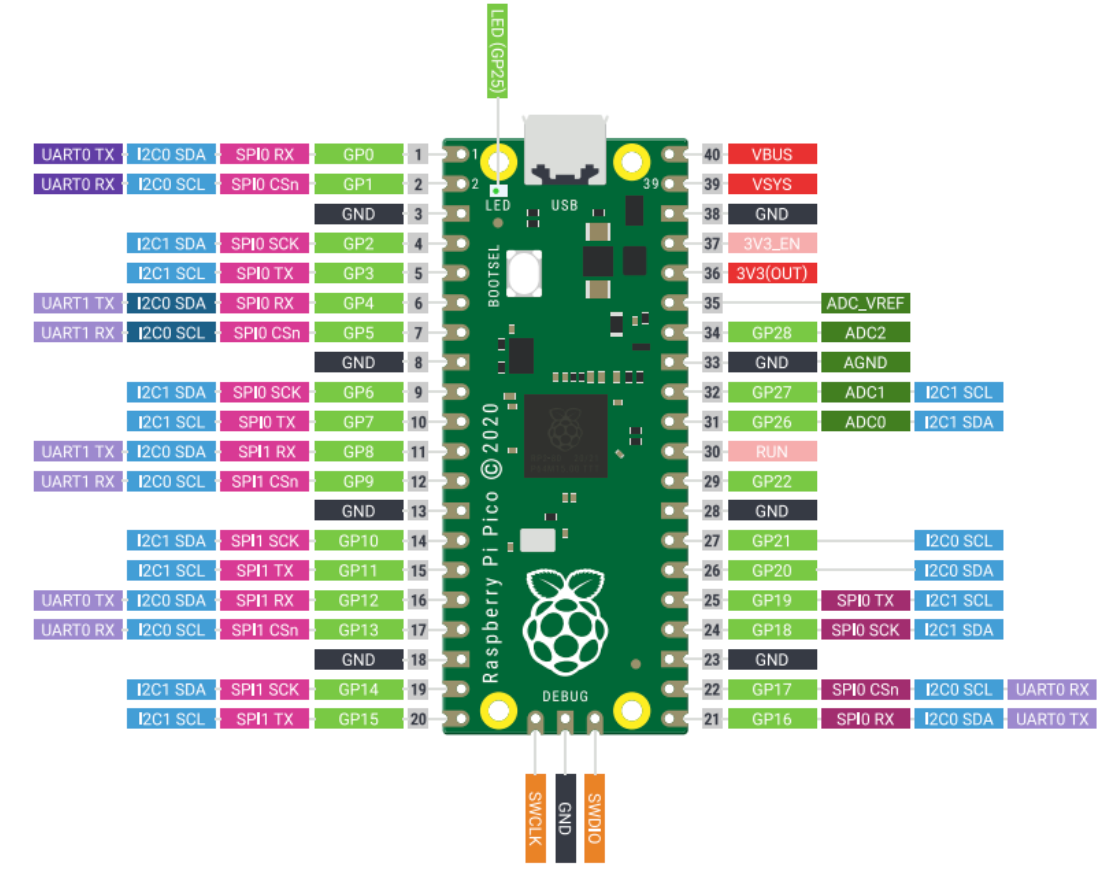
\includegraphics[width = \textwidth]{bilder/picopinout.png}
    \caption{Pico Pin Map}
    \label{fig:pico}
\end{figure}

\subsection{Ansluta till wifi och MQTT}
Raspberry Pi Picon är byggt för att klara av wifi på 2.4GHz bandet, dvs har du ett 5GHz wifi så kan det bli problem att ansluta till wifi. För att underlätta anslutning till MQTT så använd den bifogade filen $simple.py$ som är ett bibliotek för att ansluta till MQTT. Från denna fil behöver ni importera $MQTTClient$.
För att skapa en MQTT client så behövs följande information:
\begin{itemize}
    \item Id
    \item Server
    \item Port
    \item Användarnamn
    \item Lösenord
\end{itemize}

Här syftar användarnamnet och lösenordet på ert användarnamn till adafruit, samt eran Active Key. Id är namnet på er pico, det kan ni döpa till något lämpligt, Server i detta fall är "$io.adafruit.com$", port är som standard 1883 för denna MQTT.
Er klient måste sedan förses med en så kallad callback funktion, dvs en funktion som hanterar varje gång ett meddelande som enheten prenumenerar på kommer in. Det är också viktigt att tala om för enheten vilket ämne den bör prenumenera på!

Rekommenderar även i denna övning att ni håller all känslig information i ett separat dokument, se figur \ref{fig:my_label} för ett exempel på hur ett sådant kan se ut.

\begin{figure}[H]
    \centering
    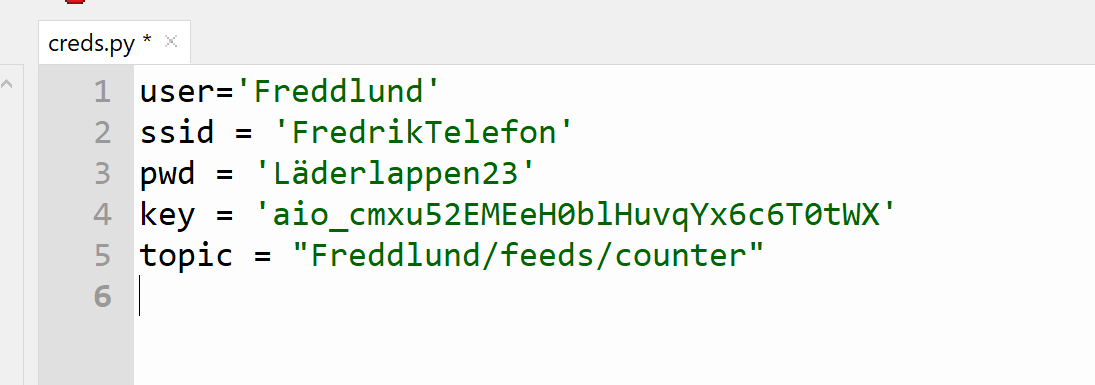
\includegraphics[width=0.8\textwidth]{exempelwifi.png}
    \caption{Exempel på hur creds fylls i.}
    \label{fig:my_label}
\end{figure}
\newpage
\subsection*{Sammanfattning}
Här kommer en sammanfattning på vad ni behöver göra i denna labben.
\begin{itemize}
    \item Koppla upp till wifi.
    \item Skapa och koppla upp en MQTT klient.
    \item Skriv kod som översätter ett decimalt tal till ett 3 bitars binärt tal.
    \item Koppla upp fysiska LEDs.
\end{itemize}
Notera att detta nödvändigtvis inte behöver vara den ordningen som ni behöver göra. Ni kan börja hur ni vill, med undantaget att Wifi behöver kopplas upp innan ni kan koppla upp till er MQTT klient.

Lycka till!

\end{document}
